\documentclass[12pt,twocolumn]{article}
\usepackage[margin=0.7in]{geometry}
\usepackage{graphicx}
\usepackage{cite}
\linespread{1.5}
                                        
%%%%%%%%%%%%%%%%%%%%%%%%%%%%%%%%%%%%%%%%%%%%%%%%%%%%%%%%%%%%%%%%%%%%%%%%%%%%%%%%%%%%%%%%%%%%%%%%%%%%%%%%%%%%%%%%%%%%%%%%%%%%%%%%%%%%%%%%%%%%%%%%%%%%%%%%%%%%%%%%%%%%%%%%%%%%%%%%%%%%%%%%%%%%%%%%%%%%%%%%
                                        
\begin{document}
\title{Single/Double Slit Experiments}
\author{M. Lane and Alex J. Harsell.}
\date{\today}

\maketitle


\begin{abstract}
Particle wave duality is one of the most perplexing concepts in modern physics. This apparent
paradox seems to defy intuition, which is built upon common experience. In this experiment the
double and single slit experiments are performed one photon at a time. It is shown that a single
photon experiences wave interference in both the single and double slit cases. In this sense the
particle and wave natures of light are shown simultaneously, which motivates the paradox of duality
in an undeniable way.
\end{abstract}

\section{Introduction}

\begin{figure}[h!]
	\centering
	\label{fig:eq}
	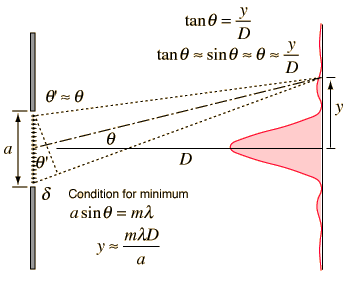
\includegraphics[width=3in]{images/sinslit.png}
	\caption{Replace picture with correct variables or picture in notes}
\end{figure}
Introduced by Albert Michelson in 1881, the Michelson Interferometer was instrumental in ushering in the era of modern physics; most notably, it validated Einstein's theory of special relativity and dismissed the omnipresence of an ether through which light was thoughtto have propagated. It's applications, however, are varied and can be used to discern wavelengths given precise measurements of distance or vice versa.[2] In addition, the Michelson Interferometer can determine the separation of wavelengths of non monochromatic light. If two wavelengths are present, they will "beat" in the same way that two closely separated audio waves beat. Intuitively, the interference patterns for each wavelgength present in the extended source superimposes and will thus rotate in phase and out of phase as the path lengths are altered.
Superposition in this manner is true for arbitrarily contiguous light sources. The final application demonstrated in this study is the present of white light fringes which should exist in theory since there is a point where all waves intefere, irrespective of wavelength.[2]
\section{Theory}
\begin{figure}[h!]
	\centering
	\label{fig:setup}
	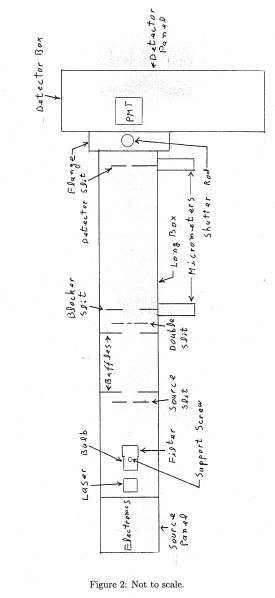
\includegraphics[width=3in]{images/Labphoto1}
	\caption{Results for Two Slit with Laser}
\end{figure}
Interference is one of the many significant consequences of the wave nature of light. Fortunately, these efeffects are also accessible, many of them are presented in an introductory physics course. The Michelson Interferometer is a practical way of superimposing two light sources to ob- serve interference. A schematic from Guenther's Modern Optics is shown in figure 1.[1] After passage through a
beam splitter the primary ray of light moves along two orthogonal paths (the arms of the interferometer) before rejoining to produce an inteference pattern observed at the detector. $M^2_{O}$ is the location of the virtual image of $M_2$ seen through the beam splitter. $M_2$ and $M0_2$ are equidistant from the beam splitter. The beams on each arm react from $M_1$ and $M_ 2$ identically so that both beams experience the same $\pi$ phase change. Also, we assume that the entire apparatus is encased in air which has a dielectric constant approximately equal to unity.
The difference in path lengths for parallel rays traversing each arm is given by |2d| since the light must travel to and back. Unfortunately, the rays incident on the detector are not all parallel; the rays in general are refected at an angle $\theta$ away from the center. Thus, the optical
path length difference between the two arms is $2d cos \theta$ and modern optics dictate that maxima in the inteference pattern occur when
$2d cos theta = m\lamda$ (1)
where m is an integer and  is the wavelength.[2] Note that in equation 1, we have assumed that the light source is monochromatic. Also, we note that given a constant d, m, and , cos  is constant, thus, these maxima and
hence, the fringes between the maxima, are spherically symmetric. As we vary d linearly, m varies linearly as well (albeit discreetly) so that a ring of maximal intensity dis- appears when $2d$ descreases by $\lambda$ and appears when 2d is increased by $lamda$. In this way, we can measure distances on the order of the wavelength of the light source or measure the wavelength of the light source by varying the position of $M_1$ by a known quantity and counting fringes that appear or disappear, depending on the direction moved. If we x our observation to a central reference point on the detector, we have that
d =(n)2(2)
where d is the change in displacement of M1 and where n is the number of fringes passing the reference point. Now, we consider the case for when there are two wavelengths, 1 and 2 present in a dichromatic light source. The two inteference patterns are dictated by equation 1 and are superimposed at the detector. The maxima in the combined inteference patterns then, occur at displacements when each separate  interference pattern is maximized, that is, when the optical path dierence is an integer multiple of both 1 and 2. The minima of the combined inteference patterns occur directly between the maxima for symmetry reasons. Suppose we have found a displacement d1 which gives maximal fringe visibility in the  eld of view. Then, the next displacement which gives maximal fringe visibility occurs when
 2(d2 d1) = n1 = (n + 1)2 (3)
 for some integer n. In words, we require that the shorter wavelength wave shift one fringe more than the more slowly varying long wavelength in the course of a full period of beats. We can solve equation 3 for n as
n =21  2(4)

and subsequent substitution of equation 4 back into equa-
tion 3 gives
1  2 =
12
2(d2  d1)
=
12
2d
(5)
Let us denote 
as the average wavelength. Then, 2 
1 = 2 and 2  2 = 1. If the wavelength separation
is small, we dene the small quantities   1 and  
  2. Assuming the intensities of the two wavelengths
are equal, we have  = . Then
12 = ( + )( + )
= 2
+  +  + 
= 2
 
2
 
2
to good approximation so that

1  2 =

2
2d
(6)
This gives a way of determining the wavelength separa-
tion given the average of the wavelength. If it is assumed
that the intensities are approximately the same, then the
average is centered between 1 and 2.
Finally, we discuss the possibility of the observation
of white light fringes with the Michelson Interferometer.
We rst observe that equation 1 is wavelength indepen-
dent only when d = 0, that is, when M1 coincides with
M0
2
. It is at this zero optical path dierence that fringe
eects for white light are observed, since white light con-
tains a range of wavelengths from 400 nm to 750 nm.[1, 2]
As M1 is displaced from M0
2
, however, the fringes of dif-
ferent colors begin to separate until after roughly 8 to 10
fringes, many colors persist at any particular point, wash-
ing out the fringe pattern. Note that the presence of the
compensating plate is crucial in this analysis so that the
light travels through glass three times regardless of which
path it takes.[2]
\section{Method}
Figure 2 is picture of the apparatus used in this experiment taken onsite. The moveable mirror M1 is controlled by a lever arm attached to an adjustable micrometer. The light sources used were a standard mercury lamp and white light source. To isolate specic bandwidths of the mercury spectrum, a green or yellow lter was placed between the source and the beam splitter. M2 is tilt-adjustable with two screws at opposite corners and spring tension at a third corner. The center of the eye-piece is marked by a reference dot denoting the center of the field of view. The experiment was divided into three parts as outlined by the Physics 410 experiment reference packet.[3] First, fringes passing the reference point were counted.  
nction of micrometer displacement for mercury green light. A picture of these fringes and the reference point is given in gure 3. A course ruler measurement was used to ensure that the readings corresponded to theory. Then, the known mercury green line wavelength was used to calibrate the screw and determine the screw error
Next, the green lter was replaced by the yellow lter
to observe the yellow mercury wavelength doublet. The
calibrated micrometer could then be used to measure the
displacement required to move from one region of fringe
non-visibility to the next.
Finally, the mercury source was swapped with a white light source with all lters removed and white light fringes were observed at the displacement which satisfied the zero optical path length difference condition.
\section{DataTable}
	first paper look in
\section{Analysis}
To determine the wavelength of mercury, we rst need to determine how a degree change in the micrometer cor- responds to displacement of the moveable error. Rotation ...
micrometer by a full twenty degrees translates the
mirror by 5=32  1=128ths of an inch. This coarse mea-
surement gives the correspondance of 200  10 m per
degree. The average number of subdegrees required for
fty fringes to pass is 6:7  :3 using data from table I,
assuming a Gaussian distribution. In microns, this is ap-
proximately 13:4  0:9 m and from equation 2, we have
orresponds to within :02% of the accepted wave-
length of mercury's green line, 546:0735(5) nm.
Usually, it is prudent to use the accepted value for the
mercury green spectral line to calibrate the screw ratio,
since a ruler measurement can't be expected to produce
accurate data for displacements on the order of microns.
The wavelength of the mercury green line is accepted to
be 546:073(5) nm.[4] Using an average of 6:7  :3" per
50 fringes passing the reference point, we use equation 2
again to compute a ratio of 204  9 m per degree. The
uncertainty margin here is similar to that produced by
e ruler measurement indicating that the uncertainty
in counting is similar to the uncertainty introduced in
measuring distances with a precision ruler.
Next, we compute the average of the separations of
table II as 40  2", again assuming a Gaussian distri-
bution. In microns, the separation distance is given by
81:6  5:4 m. Given that the average wavelength of
the mercury yellow lines is 578:013(5) nm[4], we can use
equation 6 to compute the separation.
1  2 
578:013
2
2  81600
= 2:05  :14 nm (8)
so that one line has a wavelength of approximately
579:04  0:07 nm and the other line has wavelength ap-
proximately 576:99  0:07 nm. All uncertainty estimates
in this section were determined via standard error propa-
gation procedures and we relegate assessments of uncer-
tainty and possible systematic uncertainty to the next
section.
The white fringes can be reproduced consistently after
a few tries. The approximate range over which they are
visible is 1:5" so the micrometer needs to be adjusted
very slowly when searching for them. The number of
white fringes visible in this interferometer agrees with
Jenkins & White; in general, they report that 8 to 10
fringes are visible on each side of the central fringe.[2]
...
\section{Error}
 that f = :14 nm as reported. Other uncertainties are
computed in like manner.
As the device itself is fairly simple, there are few
problems that might cause global systematic uncertain-
ties. The most signicant of such eects is the backlash
present in the micrometer. Care was taken throughout
the experiment to continue to rotate the micrometer in
one direction. However, due to the nature of the record-
taking, the micrometer motion needed to be stopped at
each measurement. Thus, we can expect distance mea-
surements to vary an additional quarter of a subdegree
or about half a micron.

\begin{figure}[h!]
	\centering
	\label{fig:2slit}
	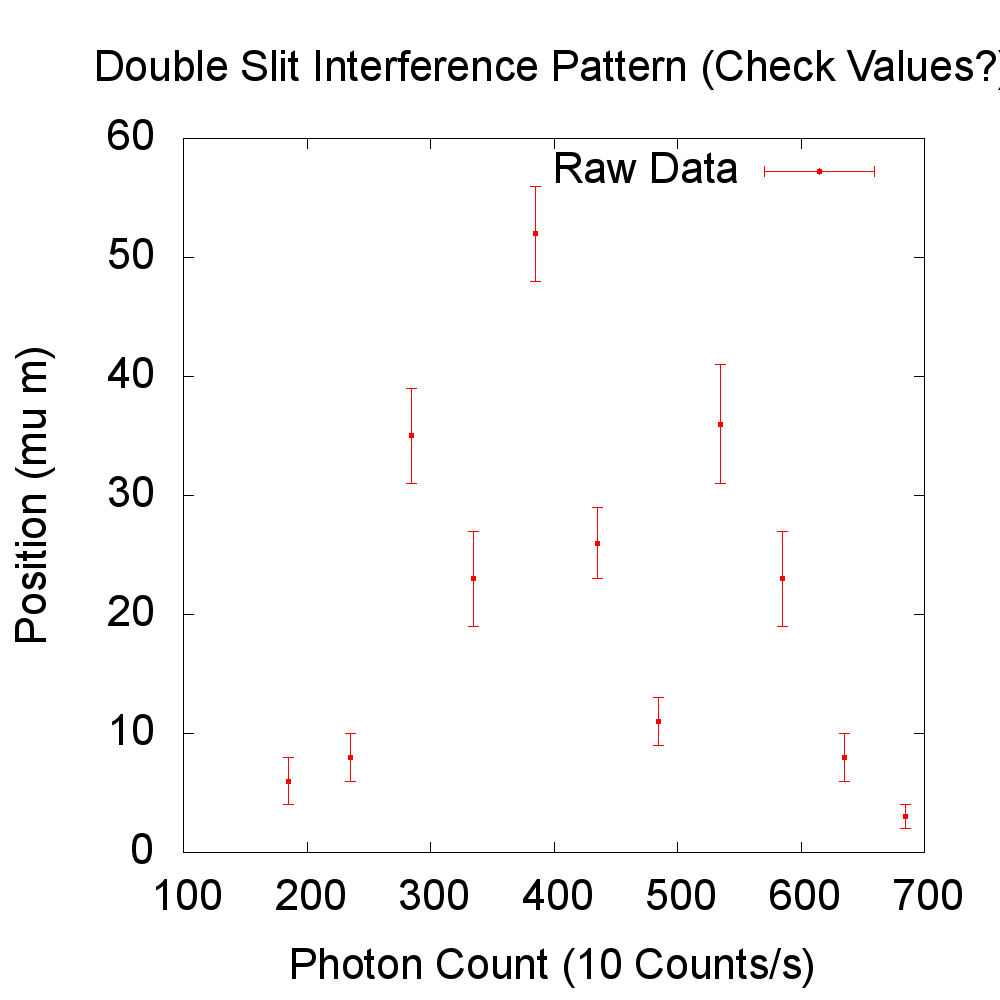
\includegraphics[width=3in]{images/Twoslit}
	\caption{Results for Two Slit with Laser}
\end{figure}
\begin{figure}[h!]
	\centering
	\label{fig:1slit}
	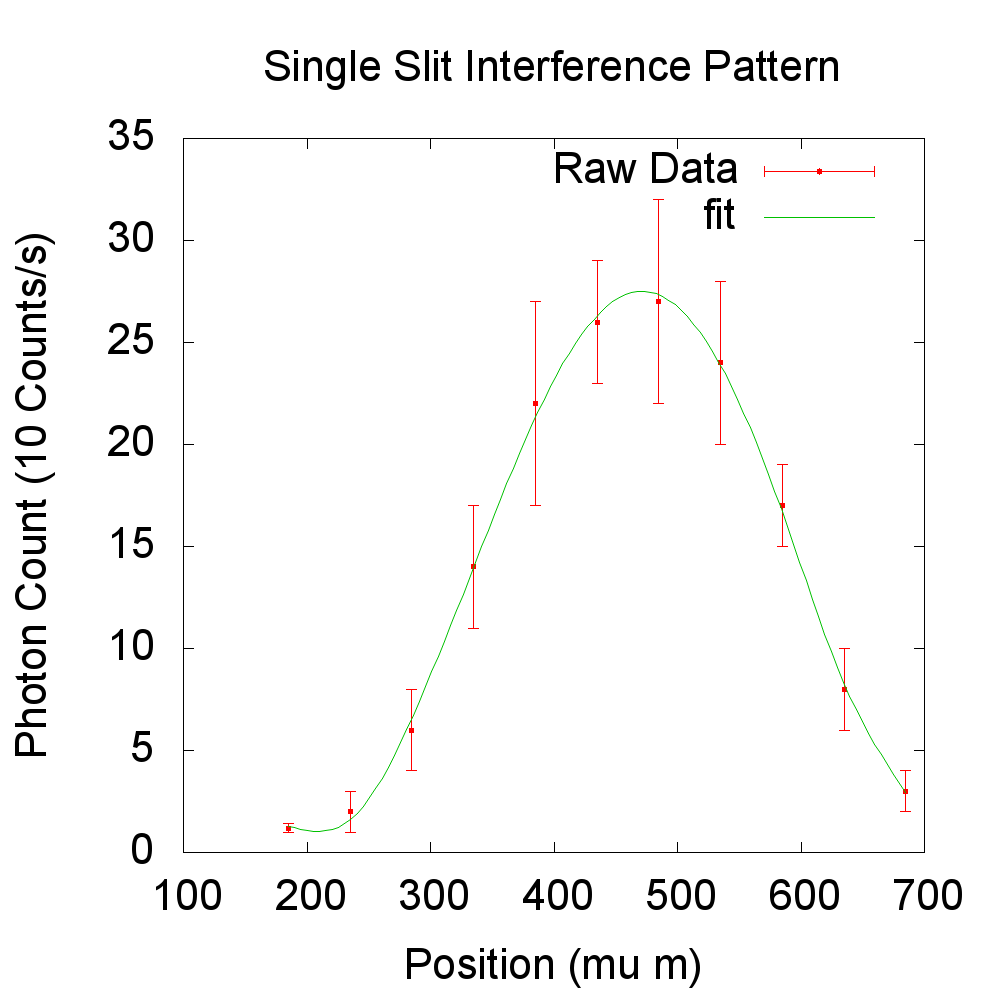
\includegraphics[width=3in]{images/Oneslit}
	\caption{Results for One Slit with Laser}
\end{figure}
\section{Conclusion}
In conclusion, the experiments both determined val-
ues for the mercury green and yellow line wavelengths
to great accuracy and demonstrated the existence of
white light fringes. The mercury green line is reported
to be 540  36theo  10sys nm in agreement with the
accepted value, 546:0735(5) nm.[4] The mercury yellow
lines from experiment are 576:99  0:07theo  0:04sys nm
and 579:040:07theo0:04sys nm in agreement with their
accepted values, 576:9598(5) nm and 579:0663(5) nm, as
4] Finally, the number of visible white light fringes
corresponds roughly to the number of fringes expected
in Jenkins & White and our experiment is in agreement
with standard optics theory
\nocite{*}
\bibliography{references}
\bibliographystyle{plain}
\section{Extra Biography}
[1] M. Sobel, Light (The University of Chicago Press, 1987), pp. 8-15.
[2] P. Tipler, R. Llewellyn Modern Physics (W.H. Freeman Company 1999,2003), pp. 141-143.
[3] R. Feynman, The Character of Physical Law (MIT Press 1967) pp. 128.
[4] D. Halliday, R. Resnick, J. Walker, Fundamental of Physics Volume 2 (John Wiley and Sons,
Inc., 2005), pp 996-1003.
[5] R. Feynman, Quantum Electrodynamics (Oxford University Press, 1988), pp. 78.

\end{document}
